\documentclass{article}
\usepackage{graphicx}
\usepackage{amsmath}
\usepackage{listings}
\usepackage{xcolor}
\usepackage{hyperref}
\usepackage{listings}
\usepackage{fancyhdr}
\usepackage[a4paper, hmargin = 1.5cm, head = 4cm, bottom = 2cm]{geometry}

\lstdefinestyle{javastyle}{
    language=Java,
    basicstyle=\ttfamily,
    numbers=left,
    numberstyle=\tiny,
    numbersep=5pt,
    frame=single,
    breaklines=true,
    captionpos=b,
    keywordstyle=\color{blue},
    commentstyle=\color{green!50!black},
    stringstyle=\color{red},
}



\lstdefinestyle{mystyle}{
    basicstyle=\ttfamily,
    numbers=left,
    numberstyle=\tiny,
    numbersep=5pt,
    frame=single,
    breaklines=true,
    captionpos=b,
    keywordstyle=\color{blue},
    commentstyle=\color{green!50!black},
    stringstyle=\color{red},
}

\lstdefinelanguage{MyPython}{
    language=Python,
    basicstyle=\ttfamily,
    morekeywords={print,for,if,else},
}


\lstdefinestyle{haskellstyle}{
    language=Haskell,
    basicstyle=\ttfamily,
    numbers=left,
    numberstyle=\tiny,
    numbersep=5pt,
    frame=single,
    breaklines=true,
    captionpos=b,
    keywordstyle=\color{blue},
    commentstyle=\color{green!50!black},
    stringstyle=\color{red},
}


\lstset{style=mystyle}


\begin{document}


\pagestyle{fancy}
\lhead{\includegraphics[width=0.27\textwidth]{assets/eth_logo.pdf}}
\rhead{Formal Methods and Functional Programming}
\lfoot{Spring Semester 2023}
\rfoot{\thepage}
\cfoot{}
\renewcommand{\footrulewidth}{1pt}


\begin{titlepage}
    \thispagestyle{fancy}
    \renewcommand{\headrulewidth}{1pt}

    \center
    \vspace*{1.0cm}
    \Large Formal Methods and Functional Programming \\[.5 cm]
    \large
    \normalsize
    Gnkgo, Informatik B. Sc. 4. Semester \\
    \vfill
\end{titlepage}

% Table of Contents
\tableofcontents
\newpage % Start content on a new page
\tableofcontents 


\section{Haskell}

\subsection{Input/Output}

Java code:

\begin{lstlisting}[style=javastyle, caption=Java Code, label=code:java]
void f(String out) {
    String inp1 = Console.readLine();
    String inp2 = Console.readLine();
    if (inp2.equals(inp1)) System.out.println(out);
}
\end{lstlisting}
How to convert to Haskell:
\begin{lstlisting}[style=haskellstyle, caption=Haskell Code, label=code:haskell]
f :: String -> IO ()
f out = do
inp1 <- getLine
inp2 <- getLine
if inp2 == inp1
    then putStrLn out
    else return ()
\end{lstlisting}

\subsection{Syntax for IO type}

The syntax for the IO type includes:
\begin{itemize}
    \item The \texttt{do} block sequences side effects.
    \item \texttt{<-} extracts values from IO.
    \item \texttt{return} wraps values in IO.
    \item \texttt{show} converts values to Strings.
    \item \texttt{read} converts Strings to values (Always specify the desired type!).
    \item For $\alpha$-equivalence, no variables can be free.
\end{itemize}

\section{Syntax Tree}

The syntax tree rules include:
\begin{itemize}
    \item $\land$ binds stronger than $\lor$ and stronger than $\rightarrow$.
    \item $\rightarrow$ associates to the right; $\land$ and $\lor$ associate to the left.
    \item Negation binds stronger than binary operators.
    \item Quantifiers extend to the right as far as possible.
\end{itemize}

Proof Rule for Induction Step:

\begin{figure}[ht]
    \centering
    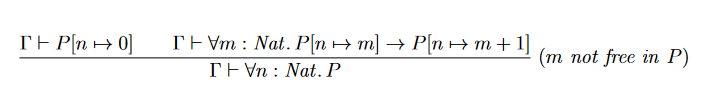
\includegraphics[width=0.5\textwidth]{assets/induction-step-tree.png}
    \caption{Induction Step Tree}
\end{figure}

\section{Foldr/Foldl}


\subsection{Foldr}



The easiest way to understand \texttt{foldr} is to rewrite the list as a series of cons operations.

\begin{lstlisting}[style=haskellstyle, caption=Haskell Code, label=code:haskell]
[1,2,3,4,5] => 1:(2:(3:(4:(5:[]))))
\end{lstlisting}

Now what \texttt{foldr f x} does is that it replaces each \texttt{:} with \texttt{f} in infix form and \texttt{[]} with \texttt{x} and evaluates the result.

For example:

\begin{lstlisting}[style=haskellstyle, caption=Haskell Code, label=code:haskell]
sum [1,2,3] = foldr (+) 0 [1,2,3]
\end{lstlisting}

\texttt{[1,2,3] === 1:(2:(3:[]))}

So,

\begin{lstlisting}[style=haskellstyle, caption=Haskell Code, label=code:haskell]
sum [1,2,3] === 1+(2+(3+0)) = 6
\end{lstlisting}

\section{Currying and Uncurrying}

Currying is the process of transforming a function that takes multiple arguments in a tuple as its argument into a function that takes a single argument and returns another function that accepts further arguments one by one. You can convert between curried and uncurried forms using the Prelude functions \texttt{curry} and \texttt{uncurry}.

\section{CYP}

Proof by induction on List \texttt{xs} generalizing \texttt{zs}:

\begin{lstlisting}[style=mystyle, caption=Haskell Code, label=code:haskell]
    Case []
    For fixed \texttt{zs}
    Show: \texttt{rev [] ++ zs .=. qrev [] zs}
    ...
Case y:ys
    Fix \texttt{y, ys}
    Assume
        IH: forall \texttt{zs: rev ys ++ zs .=. qrev ys zs}
    Then for fixed \texttt{zs}
    Show: \texttt{rev (y:ys) ++ zs .=. qrev (y:ys) zs}
    ...
QED
\end{lstlisting}

\section{$\eta$-conversion}

The following two terms are equivalent under $\eta$-conversion:

\[
x \rightarrow f x \text{ and } f
\]
Converting from left to right is $\eta$-contraction, and converting from right to left is $\eta$-expansion. $\eta$-conversion is sometimes useful to simplify expressions.
Example:
Function \texttt{parity} takes a list of Integers and transforms it into a list of 0/1s.
\begin{lstlisting}[style=haskellstyle, caption=Haskell Code, label=code:haskell]
parity xs = map elemPar xs where elemPar x = mod x 
\end{lstlisting}

\section*{General Procedure of \texttt{foldr} and \texttt{foldl}}

1. Identify recursive, dynamic, and static arguments.

\begin{lstlisting}[style=haskellstyle, caption=Haskell Code, label=code:haskell]
foldl f z (x:xs) = foldl f (f z x) xs
\end{lstlisting}
2. Write an auxiliary function that has the recursive, then the dynamic arguments. Static arguments can still occur freely (and will come from the final context).
\begin{lstlisting}[style=haskellstyle, caption=Haskell Code, label=code:haskell]
aux [] z = z
aux (x:xs) z = aux xs (f z x)
\end{lstlisting}
3. Write the dynamic arguments as lambdas.
\begin{lstlisting}[style=haskellstyle, caption=Haskell Code, label=code:haskell]
aux [] = \z -> z
aux (x:xs) = \z -> aux xs (f z x)
\end{lstlisting}
4. Rewrite \texttt{aux} in terms of \texttt{foldr}. \texttt{x} and \texttt{aux xs} become arguments of the function for the recursive case.
\begin{lstlisting}[style=haskellstyle, caption=Haskell Code, label=code:haskell]
aux = foldr (\x rec -> \z -> rec (f z x)) (\z -> z)
\end{lstlisting}
5. Express the original function in terms of \texttt{aux} (reorder the dynamic and recursive arguments, if needed).
\begin{lstlisting}[style=haskellstyle, caption=Haskell Code, label=code:haskell]
foldl f z xs = aux xs z
\end{lstlisting}
6. Replace \texttt{aux} with its implementation.
\begin{lstlisting}[style=haskellstyle, caption=Haskell Code, label=code:haskell]
foldl f z xs = foldr (\x rec z -> rec (f z x)) (\z -> z) xs z
\end{lstlisting}
\section{IMP}

Remember the following:
\begin{figure}[ht]
    \centering
    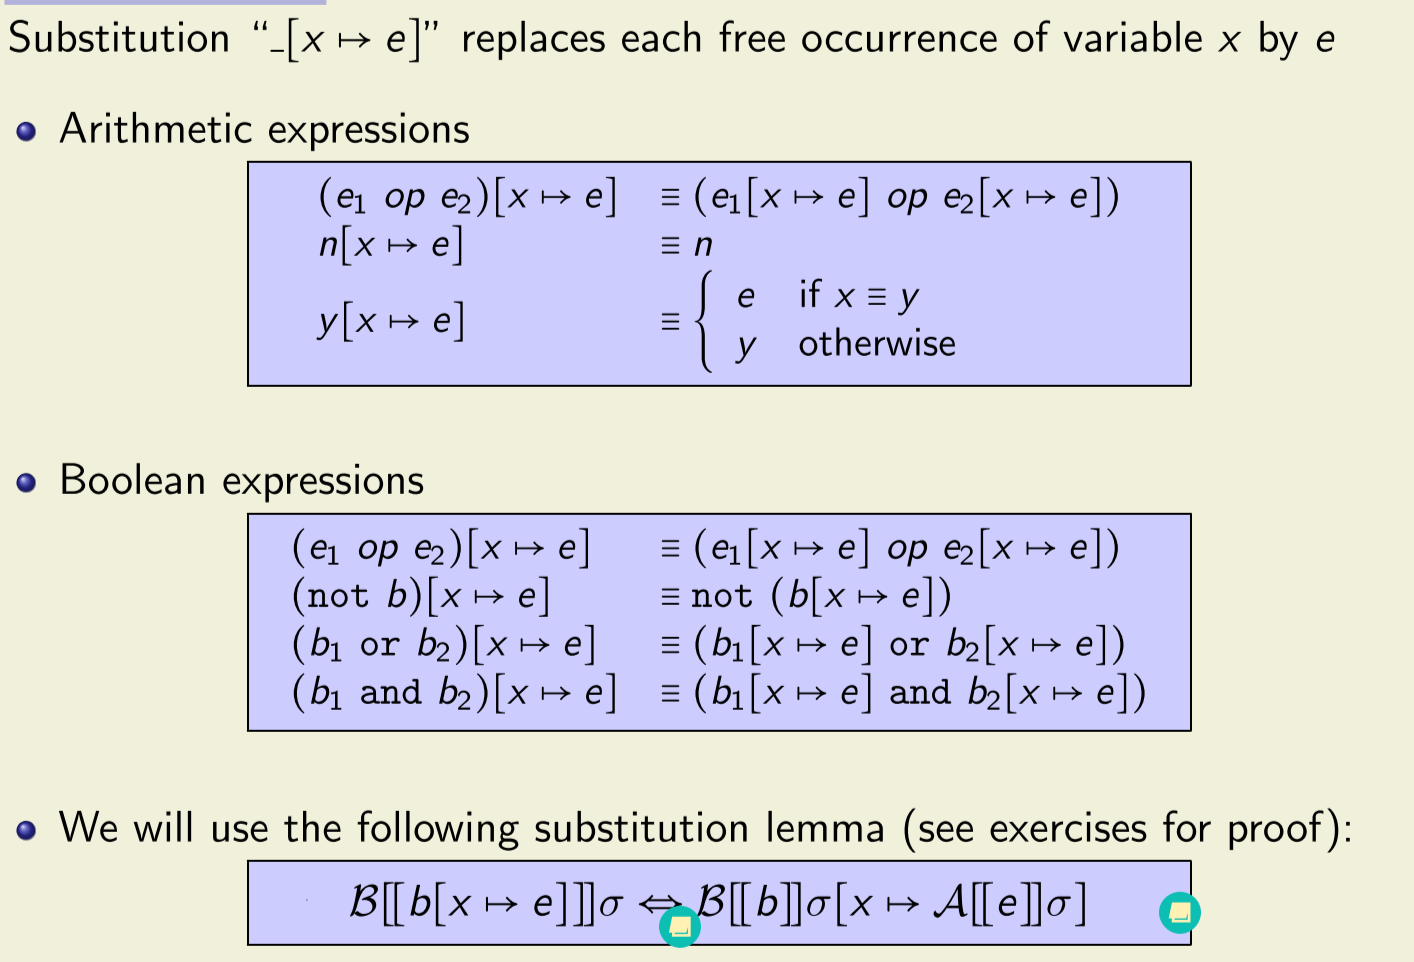
\includegraphics[width=0.5\textwidth]{assets/substitution-rule.png}
    \caption{Substitution Rule}
\end{figure}

\begin{figure}[ht]
    \centering
    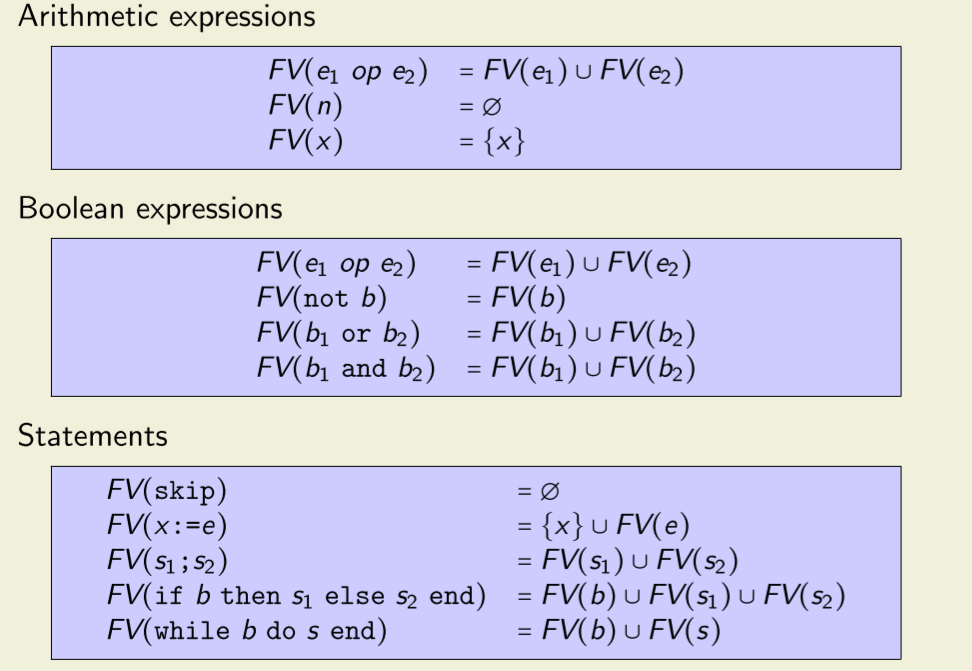
\includegraphics[width=0.5\textwidth]{assets/free-variable.png}
    \caption{Free Variable}
\end{figure}

\subsection{Proof Structure}

\subsubsection{Free Variables / Arithmetic Expression}

Let $x, y$ be arbitrary. Use strong structural induction on $e$. Thus, we have to prove $P(e)$ for some arbitrary arithmetic expression $e$ and assume $\forall e'' \subset e, P(e'')$ as our induction hypothesis.
- \textbf{Case 1:} $e \equiv n$ for some numerical value $n$.
- \textbf{Case 2:} $e \equiv y$ for some variable $y$.
- \textbf{Case 3:} $e \equiv e_1 \text{ op } e_2$ for some arithmetic expression $e_1, e_2$ and some arithmetic operator $op$.

\subsubsection{Boolean Expression}

- \textbf{Case 1:} $b \equiv b_1 \text{ or } b_2$ for some boolean expressions $b_1, b_2$.
- \textbf{Case 2:} $b \equiv b_1 \text{ and } b_2$ for some boolean expressions $b_1, b_2$.
- \textbf{Case 3:} $b \equiv \text{not } b'$ for some boolean expression $b'$.
- \textbf{Case 4:} $b \equiv e_1 \text{ op } e_2$ for some arithmetic expression $e_1, e_2$ and some arithmetic operator $op$.

\subsubsection{Trees}

$R[T] \equiv \forall T, P, Q, b, s... \text{ root}(T) \equiv ... \implies ...$
We want to prove $\forall T.R(T)$ by strong induction over the shape of $T$. Assume $\forall T' \subset T.R[T']$. Assume LHS holds. We do a case distinction on the last rule applied in $T$:
\begin{verbatim}
Here goes the proof

   \         T1          /
    \                   /
     -------------------
            X, Y
\end{verbatim}
Since $T1 \subset T$, and the root has the same statement, we can apply the I.H. We instantiate $P, Q,...$ as $P', Q',...$ respectively. Since LHS holds, we know $\exists T'$ s.t. $\text{root}(T') \equiv ...$.
\section{Find Invariants}

\subsection{Min, Max (continued)}

\begin{lstlisting}[style=mystyle, caption=Haskell Code, label=code:haskell]
while (x < y) {
    t := x; 
    x := y;
    y := t
}
\end{lstlisting}

$\{\downarrow x = \max(X, Y)\}$

Invariant: $\{ \max(x, y) = \max(X, Y) \}$

Variant: $y - x = Z$

\subsection{Swap}
Let $x \geq 0$ and $x = X$.
\begin{lstlisting}[style=mystyle, caption=Haskell Code, label=code:haskell]
a := x;
y := 0;
while (a \neq 0) {
    y := y + 1;
    a := a - 1;
}
\end{lstlisting}
$\{\downarrow y = X\}$
Invariant: $\{ a + y = X \land a \geq 0 \}$
Variant: $a$
\subsection{$A^{2^N}$}
$\{ a = A \land A > 0 \land n = N \land N \geq 0 \}$
\begin{lstlisting}[style=mystyle, caption=Haskell Code, label=code:haskell]
k := 0;
r := a;
while (k < n) {
    k := k + 1;
    r := r \cdot r
}
\end{lstlisting}

$\{\downarrow r = A^{2^N}\}$
Invariant: $\{ a = A \land A > 0 \land n = N \land N \geq 0 \land r = A^{2^k} \land k \leq N \}$
Variant: $n - k$
\subsection{Remainder}
$\{ N \geq 0 \land D > 0 \land d = D \land r = N \land q = 0 \}$

\begin{lstlisting}[style=mystyle, caption=Haskell Code, label=code:haskell]
while (r \geq 0) { 
    r := r - d; 
    q := q + 1;
} 
r := r + d;
q := q - 1;
\end{lstlisting}
$\{\downarrow N = q \cdot D + r \land r \geq 0 \land r < D\}$
Invariant: $\{ N = q \cdot d + r \land d = D \land D > 0 \land r + d \geq 0 \}$
Variant: $r = Z$
\subsection{$N^K$}
$\{ k \geq 1 \land k = K \land n \geq 1 \land n = N \}$

\begin{lstlisting}[style=mystyle, caption=Haskell Code, label=code:haskell]
i := 0;
r := 1;
while (i < k) {
    i := i + 1;
    r := r \cdot n;
}
\end{lstlisting}

$\{\downarrow r = N^K\}$
Invariant: $\{ k = K \land n = N \land r = n^i \land i \leq k \}$
Variant: $k - i = V$
\subsection{$N = q \cdot D + r$}

$\{ N \geq 0 \land D > 0 \land d = D \land r = N \land q = 0 \}$
\begin{lstlisting}[style=mystyle, caption=Haskell Code, label=code:haskell]
while (r \geq 0) {
    r := r - d;
    q := q + 1;
}
r := r + d;
q := q - 1;
\end{lstlisting}
Use the loop invariant in the invariant.
Use post-condition in the loop invariant.
Check if you can already conclude with the invariant your post-condition.
\section{Liveness and Safety}
\textbf{Liveness}
\begin{itemize}
    \item Something good will happen eventually.
    \item If the good thing has not happened yet, it could happen in the future.
    \item A liveness property does not rule out any prefix.
    \item Every finite prefix can be extended to an infinite sequence that is in $P$.
    \item Liveness properties are violated in infinite time.
\end{itemize}
\textbf{Safety}
\begin{itemize}
    \item Something bad is never allowed to happen (and can't be fixed).
    \item Safety properties are violated in finite time and cannot be repaired.
\end{itemize}

\end{document}
